% !TeX program = xelatex
% Compile with XeLaTeX (twice) or Tectonic. See README_EN.md.
\documentclass[aspectratio=169,10pt]{beamer}
\usepackage{fontspec}
\usepackage{tikz,booktabs,tabularx,colortbl}
\usetikzlibrary{arrows.meta,positioning,calc}
\setsansfont[BoldFont=texgyreheros-bold.otf,ItalicFont=texgyreheros-italic.otf]{texgyreheros-regular.otf}
\definecolor{Navy}{HTML}{17354C}
\definecolor{Teal}{HTML}{147D80}
\definecolor{Amber}{HTML}{C88722}
\definecolor{Rose}{HTML}{B95B58}
\definecolor{Muted}{HTML}{617783}
\definecolor{Soft}{HTML}{EEF4F6}
\setbeamercolor{normal text}{fg=Navy,bg=white}
\setbeamercolor{frametitle}{fg=Navy,bg=white}
\setbeamercolor{structure}{fg=Teal}
\setbeamercolor{block title}{fg=Navy,bg=Soft}
\setbeamercolor{block body}{fg=Navy,bg=Soft!55}
\setbeamercolor{takeaway}{fg=Navy,bg=Soft}
\setbeamerfont{frametitle}{size=\fontsize{18}{22}\selectfont,series=\bfseries}
\setbeamerfont{block title}{size=\normalsize,series=\bfseries}
\setbeamersize{text margin left=9mm,text margin right=9mm}
\setbeamertemplate{navigation symbols}{}
\setbeamertemplate{itemize items}{\color{Teal}\small\textbullet}
\setbeamertemplate{frametitle}{%
  \vspace{5pt}\usebeamerfont{frametitle}\insertframetitle\par
  \vspace{3pt}{\color{Teal}\rule{18mm}{1.2pt}}\vspace{2pt}}
\setbeamertemplate{footline}{%
  \hspace{9mm}\begin{minipage}{142mm}
  {\color{Muted!35}\hrule}\vspace{3pt}
  {\fontsize{6}{8}\selectfont\color{Muted}eco\_prepro\quad |\quad Results through 2026-09-18
  \hfill\insertframenumber\,/\,\inserttotalframenumber}\vspace{4pt}
  \end{minipage}}
\newcommand{\source}[1]{\par\vfill{\fontsize{6.1}{8}\selectfont\color{Muted}#1\par}}
\newcommand{\takeaway}[1]{\vspace{5pt}\begin{beamercolorbox}[wd=\linewidth,sep=6pt]{takeaway}\small #1\end{beamercolorbox}}
\newcommand{\metric}[3]{\begin{minipage}[t]{#1}\centering
  {\fontsize{30}{34}\selectfont\bfseries\color{Teal}#2}\par\vspace{3pt}{\small #3}\end{minipage}}
\newcommand{\panel}[1]{\IfFileExists{assets/#1}{\includegraphics[width=\linewidth]{assets/#1}}{%
  \fbox{\parbox[c][33mm][c]{.96\linewidth}{\centering Local QC figure not included\par\small See README\_EN.md for assets/\detokenize{#1}}}}}
\newcolumntype{Y}{>{\raggedright\arraybackslash}X}
\setlength{\tabcolsep}{5pt}
\renewcommand{\arraystretch}{1.25}
\hypersetup{pdftitle={Echocardiography Preprocessing: Data, Methods and Results},pdfauthor={eco-prepro},colorlinks=true,urlcolor=Teal}

\begin{document}

\begin{frame}[t]
  \vspace{8mm}
  {\small\color{Teal}\bfseries DATA / METHODOLOGY / RESULTS}\par\vspace{4mm}
  {\fontsize{25}{31}\selectfont\bfseries Echocardiography Preprocessing}\par\vspace{2mm}
  {\fontsize{15}{20}\selectfont Standardizing heterogeneous ultrasound inputs}\par\vspace{8mm}
  \metric{.31\linewidth}{42}{processed audit entries}\hfill
  \metric{.31\linewidth}{7,318}{total input frames}\hfill
  \metric{.31\linewidth}{7}{input sources}\par\vspace{5mm}
  \takeaway{\textbf{A deterministic pipeline for reading, region detection and standardized output.} Crop supported imaging regions; preserve uncertain and preprocessed inputs.}
  \source{Report: 2026-09-25\quad |\quad Results through 2026-09-18\quad |\quad Existing experiments; no new data runs}
\end{frame}

\begin{frame}[t]{Data processed: 42 entries from seven sources}
  \small
  \begin{tabularx}{\linewidth}{@{}l r l Y@{}}
    \rowcolor{Soft}\textbf{Source}&\textbf{N}&\textbf{Format}&\textbf{Audit focus}\\
    EV9V&11&MP4 / JPEG series&9 views, raw UI, ECG, dark sector, long cine\\
    EchoNet-Dynamic&3&AVI&Pass-through of preprocessed input\\
    EchoNet-Pediatric&4&AVI&Pediatric input and existing edge markers\\
    EchoNet-LVH&6&AVI&Large frames; differences in FPS sources\\
    CAMUS&7&NIfTI / MHD&Medical image reading and timing\\
    Unity&6&PNG&Static UI, dark sector, tinted B-mode\\
    DICOM fixtures&5&DICOM&4 noncardiac stills + 1 historical color cine\\
    \bottomrule
  \end{tabularx}
  \vspace{4pt}
  \begin{itemize}\setlength{\itemsep}{3pt}
    \item \textbf{Audit entries are not independent patients.} JPEG and MHD include derived inputs.
    \item Longest video: \textbf{3,243 frames}. The 7,318-frame total includes derived entries.
    \item Modern color Doppler, raw GE cine and vendor generalization remain untested.
  \end{itemize}
  \source{Source: fixed input manifest and processing audit tables in the project repository.}
\end{frame}

\begin{frame}[t]{Method: one pipeline for heterogeneous inputs}
  \begin{center}
  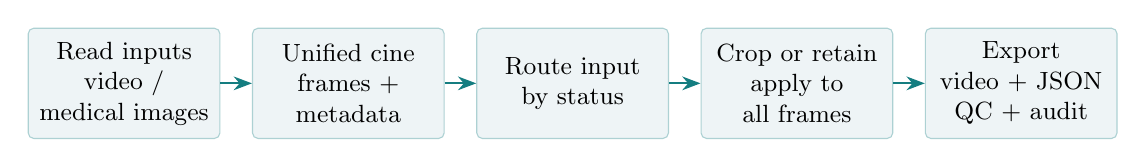
\begin{tikzpicture}[node distance=3mm and 4mm,>=Stealth,
    flow/.style={draw=Teal!35,fill=Soft,rounded corners=2pt,minimum height=14mm,text width=22mm,align=center,font=\small}]
    \node[flow] (a) {Read inputs\\video / medical images};
    \node[flow,right=of a] (b) {Unified cine\\frames + metadata};
    \node[flow,right=of b] (c) {Route input\\by status};
    \node[flow,right=of c] (d) {Crop or retain\\apply to all frames};
    \node[flow,right=of d] (e) {Export\\video + JSON\\QC + audit};
    \foreach \u/\v in {a/b,b/c,c/d,d/e}\draw[->,Teal,thick] (\u)--(\v);
  \end{tikzpicture}
  \end{center}
  \begin{columns}[T,onlytextwidth]
  \column{.31\textwidth}
    \begin{block}{Preprocessed input}\small Preserve the existing pixels and canvas.\end{block}
  \column{.31\textwidth}
    \begin{block}{Reliable moving cine}\small Detect the region, then mask, crop and square-pad.\end{block}
  \column{.34\textwidth}
    \begin{block}{Uncertain / special input}\small Retain low-confidence, static and multi-region inputs for review.\end{block}
  \end{columns}
  \vspace{3pt}\small
  \begin{itemize}\setlength{\itemsep}{4pt}
    \item SHA-256 identifies each input; record dimensions, frame count and source metadata.
    \item Keep container FPS, dataset-table FPS and the selected timing source separately.
    \item Export every frame, with the applied mask, processing status and QC evidence recorded.
  \end{itemize}
  \source{Implementation: project readers, Cine representation, standardizer and audit/export modules.}
\end{frame}

\begin{frame}[t]{Detection: motion and intensity support}
  \begin{columns}[T,onlytextwidth]
  \column{.43\textwidth}
    \begin{block}{Temporal evidence}\small
      Use up to 64 uniformly sampled frames:
      \[
        M(x,y)=\operatorname{std}_{t}\bigl[I_t(x,y)\bigr].
      \]
      Motion identifies candidate locations.
    \end{block}
  \column{.53\textwidth}
    \begin{block}{Connected imaging support}\small
      Grow candidates through connected intensity support to include near-static tissue.\\[5pt]
      Morphology removes small fragments; a convex hull provides a fallback boundary.
    \end{block}
  \end{columns}
  \vspace{5pt}
  \begin{center}
  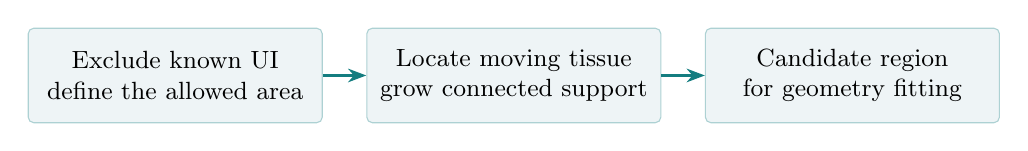
\begin{tikzpicture}[>=Stealth,box/.style={fill=Soft,draw=Teal!35,rounded corners=2pt,text width=35mm,minimum height=12mm,align=center,font=\small}]
    \node[box] (a) at (0,0) {Exclude known UI\\define the allowed area};
    \node[box] (b) at (4.3,0) {Locate moving tissue\\grow connected support};
    \node[box] (c) at (8.6,0) {Candidate region\\for geometry fitting};
    \draw[->,Teal,thick] (a)--(b);\draw[->,Teal,thick] (b)--(c);
  \end{tikzpicture}
  \end{center}
  \small\textbf{Verified EV9V layout:} exclude top text, grayscale bar, outer depth ticks and ECG. The 320$\times$240 profile is checked against image evidence.
  \source{Source: motion detector and layout exclusions in echoprep/sector/. Other layouts require their own supported exclusions.}
\end{frame}

\begin{frame}[t]{Geometry fitting and reliability checks}
  \begin{center}
  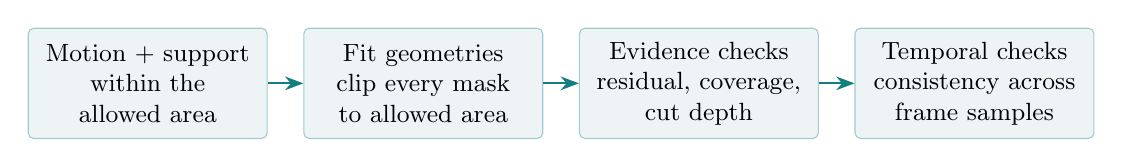
\begin{tikzpicture}[>=Stealth,box/.style={draw=Teal!40,fill=Soft,rounded corners=2pt,
      minimum height=14mm,text width=28mm,align=center,font=\small}]
    \node[box] (a) at (0,0) {Motion + support\\within the\\allowed area};
    \node[box] (b) at (3.5,0) {Fit geometries\\clip every mask\\to allowed area};
    \node[box] (c) at (7,0) {Evidence checks\\residual, coverage,\\cut depth};
    \node[box] (d) at (10.5,0) {Temporal checks\\consistency across\\frame samples};
    \foreach \u/\v in {a/b,b/c,c/d}\draw[->,Teal,thick] (\u)--(\v);
  \end{tikzpicture}
  \end{center}
  \begin{center}
  
\begin{tikzpicture}[scale=.78,sectorstyle/.style={fill=Teal!13,draw=Teal,line width=.9pt}]
    \draw[sectorstyle] (0,0)--(225:1.05) arc[start angle=225,end angle=315,radius=1.05]--cycle;
    \node[font=\small] at (0,-1.5) {Standard fan};
    \begin{scope}[shift={(4.2,0)}]
      \draw[sectorstyle] (-.22,-.22)--(225:1.05) arc[start angle=225,end angle=315,radius=1.05]--(.22,-.22)--cycle;
      \node[font=\small] at (0,-1.5) {Flat top / virtual apex};
    \end{scope}
    \begin{scope}[shift={(8.4,0)}]
      \begin{scope}[rotate=30]\draw[sectorstyle] (0,0)--(240:1.05) arc[start angle=240,end angle=300,radius=1.05]--cycle;\end{scope}
      \node[font=\small] at (0,-1.5) {Rotated wedge};
    \end{scope}
    \begin{scope}[shift={(12.6,0)}]
      \draw[sectorstyle] (-.65,-.95) rectangle (.65,-.1);
      \node[font=\small] at (0,-1.5) {Rectangle};
    \end{scope}
  \end{tikzpicture}
  \end{center}
  \small
  \textbf{Fit checks:} boundary residual, flank/arc support, retained evidence and area expansion.\\[3pt]
  \textbf{Stability:} pairwise sample-mask IoU $\geq 0.98$; IoU with the final candidate $\geq 0.97$.\\[3pt]
  \textbf{Otherwise:} use the previously trusted hull, or retain the full image if evidence is weak.
  \takeaway{One fixed mask per cine; no generated image content or fixed fan template.}
  \source{Schematics only. Flat-top, rotated single-region and rectangular moving echo: synthetic validation only.\\Source: geometry fitting and motion detector modules.}
\end{frame}

\begin{frame}[t]{Evaluation: real cases and synthetic masks}
  \begin{center}
  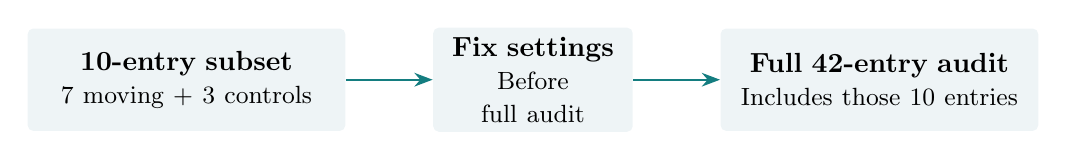
\begin{tikzpicture}[>=Stealth]
    \node[fill=Soft,rounded corners=2pt,align=center,text width=38mm,minimum height=13mm] (a) at (0,0) {\textbf{10-entry subset}\\\small 7 moving + 3 controls};
    \node[fill=Soft,rounded corners=2pt,align=center,text width=23mm,minimum height=13mm] (b) at (4.4,0) {\textbf{Fix settings}\\\small Before full audit};
    \node[fill=Soft,rounded corners=2pt,align=center,text width=38mm,minimum height=13mm] (c) at (8.8,0) {\textbf{Full 42-entry audit}\\\small Includes those 10 entries};
    \draw[->,Teal,thick] (a)--(b);\draw[->,Teal,thick] (b)--(c);
  \end{tikzpicture}
  \end{center}
  \small\renewcommand{\arraystretch}{1.15}
  \begin{tabularx}{\linewidth}{@{}l Y l@{}}
    \rowcolor{Soft}\textbf{Check}&\textbf{Setup}&\textbf{Result}\\
    Reading / export&Full decode; dimensions, frame count, FPS&42/42 passed\\
    Pixel preservation&In-memory pass-through and retained outputs&33/33 identical\\
    Synthetic geometry&Known shapes and excluded regions&Fan IoU $>0.96$\\
    Dark-gap recovery&Known synthetic missing sector segment&Gap recovery $>98\%$\\
    Temporal stability&Change sampling density and odd/even phase&Unstable fits rejected\\
    Engineering checks&Readers, retention, geometry and rejection&46 tests passed\\
    \bottomrule
  \end{tabularx}
  \takeaway{The full audit includes the tuning subset: \textbf{it is not an independent test set}. Synthetic accuracy does not establish accuracy on real images.}
  \source{Sources: recorded tests and export verification in the project repository. Pixel identity refers to in-memory output; MP4 encoding is lossy.}
\end{frame}

\begin{frame}[t]{Processing results: all 42 entries exported}
  \begin{columns}[T,onlytextwidth]
  \column{.54\textwidth}
    \small
    \begin{tabularx}{\linewidth}{@{}Y r@{}}
      \rowcolor{Soft}\textbf{Processing outcome}&\textbf{Entries}\\
      Cropped and masked&9\\
      Preprocessed input preserved&20\\
      Low confidence: retained&2\\
      Static: retained&9\\
      Multi-region flag: retained&2\\
      Runtime failure&0\\
      \bottomrule
    \end{tabularx}
  \column{.42\textwidth}
    \begin{block}{11 moving EV9V entries}
      \small\textbf{5} accepted standard-fan fits\\[4pt]
      \textbf{4} trusted hull fallbacks\\[4pt]
      \textbf{2} original images retained
    \end{block}
    \small The other \textbf{31} entries bypass geometry fitting.
  \end{columns}
  \vspace{7pt}\small
  \textbf{All 42 output videos decode fully.}\\The longest cine retains all \textbf{3,243 frames}; no frame truncation.
  \takeaway{Processing success records what the pipeline did. Visual cleanup quality is evaluated separately.}
  \source{Source: processing and export audit tables. The multi-region flag includes one unresolved false positive on a Unity still image.}
\end{frame}

\begin{frame}[t]{Temporal stability of the five accepted fits}
  \small\renewcommand{\arraystretch}{1.03}
  \begin{tabularx}{\linewidth}{@{}Y c r r@{}}
    \rowcolor{Soft}\textbf{Entry}&\textbf{Tuning subset}&\textbf{Min.\ sample IoU}&\textbf{Evidence retained}\\
    A4C&Yes&0.9943&99.73\%\\
    PLHLA&No&0.9951&99.76\%\\
    PMPALA&No&0.9937&99.60\%\\
    PPMLSA&Yes&0.9958&99.77\%\\
    3,243-frame cine&No&0.9927&99.66\%\\
    \bottomrule
  \end{tabularx}
  \vspace{2pt}
  \begin{columns}[T,onlytextwidth]
  \column{.47\textwidth}
    \begin{block}{Extent of boundary expansion}\small Fitted area vs.\ the candidate region\par\vspace{4pt}
    {\Large\bfseries\color{Teal}+3.2\% to +5.8\%}\end{block}
  \column{.49\textwidth}
    \begin{block}{What these metrics measure}\small IoU: agreement across temporal samples.\\[4pt]
    Retention: coverage of candidate evidence.\end{block}
  \end{columns}
  \takeaway{No human sector masks yet. Area expansion, stability and candidate coverage \textbf{do not measure true anatomical preservation}.}
  \source{Source: fixed processing audit table. An accepted geometry fit does not imply complete UI removal.}
\end{frame}

\begin{frame}[t]{A4C example: stable fan fit accepted}
  \panel{normal_fan.png}
  \vspace{2pt}
  \begin{columns}[T,onlytextwidth]
    \column{.30\textwidth}\small\textbf{Min.\ sample IoU}\\{\Large\color{Teal}0.9943}
    \column{.30\textwidth}\small\textbf{Evidence retained}\\{\Large\color{Teal}99.73\%}
    \column{.35\textwidth}\small\textbf{Remaining issue}\\Edge ticks and some ECG spikes may remain.
  \end{columns}
  \source{Example: ev9v\_d47d8e7414433eb2. EV9V: Bo Gou et al., CC BY 4.0; preprocessing and panel annotations by this project.}
\end{frame}

\begin{frame}[t]{Dark PASA example: original image retained}
  \panel{dark_sector.png}
  \vspace{1pt}\small
  \textbf{Reason:} insufficient flank and outer-arc evidence to infer the full sector reliably.\\[4pt]
  \textbf{Other rejections:} PMASA IoU 0.9540: hull fallback; JPEG IoU 0.8022: retain original.
  \source{Example: ev9v\_a9b7d8c2e96c23f1. EV9V: Bo Gou et al., CC BY 4.0; project-generated panel.\\Synthetic dark-gap recovery does not resolve this real dark-sector case.}
\end{frame}

\begin{frame}[t]{Visual results and current limitations}
  \begin{center}
  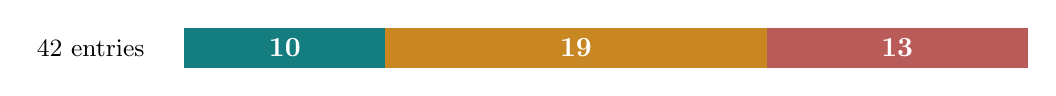
\begin{tikzpicture}[x=.255cm,y=.9cm]
    \node[anchor=east,font=\small] at (-1.5,.28) {42 entries};
    \fill[Teal] (0,0) rectangle (10,.57);
    \fill[Amber] (10,0) rectangle (29,.57);
    \fill[Rose] (29,0) rectangle (42,.57);
    \node[text=white,font=\bfseries] at (5,.285) {10};
    \node[text=white,font=\bfseries] at (19.5,.285) {19};
    \node[text=white,font=\bfseries] at (35.5,.285) {13};
  \end{tikzpicture}\par\vspace{4pt}
  {\small\color{Teal}PASS}\quad
  {\small\color{Amber}MINOR ISSUE}\quad
  {\small\color{Rose}FAIL}
  \end{center}
  \small
  \begin{itemize}\setlength{\itemsep}{5pt}
    \item \textbf{19 minor issues:} edge ticks, thin lines, ECG spikes and existing input markers.
    \item \textbf{13 FAIL entries:} unresolved raw inputs correctly retained; not runtime failures.
    \item Real dark sectors, static/multi-region screens and modern color Doppler remain unresolved or unvalidated.
    \item Ratings come from AI-assistant review of panels and first/middle/last output frames. Independent human ratings and sector masks are still missing.
  \end{itemize}
  \takeaway{The pipeline is operational and five fits are stable. \textbf{Overall visual ratings have not improved over the hull-based baseline}; anatomical accuracy remains unmeasured.}
  \source{Source: recorded visual QC tables. True flat-top, rotated single-region and rectangular moving echo remain validated only on synthetic inputs.}
\end{frame}

\end{document}
